\chapter{Analysis}

\section{Introduction}

Client: Neil Green
Job Description: Owns and manages an Independently run gym
Contact Information: Sweat Gymnasium LLP
					 107a Clay Street
					 Soham
					 Ely
					 Cambridgeshire
					 CB7 5HL

					 Telephone: 01353 721864
					 Email: info@sweatgym.co.uk

\subsection{Client Identification}

My client is an independent gym owner who is struggling to keep track of his members payment details and use of the facilities. He is also my brother in law. He approached me about creating a system for him after I mentioned I needed a client for coursework and he mentioned that he is having issues with clients not paying him since he doesn't have an accurate, reliable system for keeping track of payments.

\subsection{Define the current system}

His current system involves using a series of excel spreadsheets to document his clients payment, membership details, personal details and exercise plans. He does this manually by creating new spreadsheets and entering the clients data by hand. His clients give him this data by filling out a membership form and membership agreement and via discussion and interview if they need an exercise program made for them. My client uses one spreadsheet to keep a record of all the members of the gym including details like their member ID, their contact information, payment information and their membership details as well as whether their up to date with payments. Each member then has their own spreadsheet which is used to keep track of any exercise routines they may have paid to have planned for them.

\subsection{Describe the problems}

This system imposes some limitations. First of all, all the processes have to be dealt with manually through spreadsheets without anything other than lack of human error to point out a mistake or notify if someone isn't up to date with payment. This also isn't secure as any piece of information can be changed at any time and to be sure of everything debit mandates would have to be looked over, but even then some clients may have payed by cash and thus wouldn't be recoverable. Their is also the possibility of a computer error that could delete all the documents as they are not backed up anywhere. His gym also know accommodates over 1000 members meaning that he has a large number of spreadsheets for all his clients as well as having his main spreadsheet being exceptionally large meaning the program can lag, especially since the program isn't running on the greatest available hardware. Another issue is that it can be difficult to sort through and search the spreadsheets to find specific information regarding clients, for example if he needs to find they're contact information, excel doesn't have a tool to easily search for that.

\subsection{Section appendix}

Q. What is your current system?

Our current system involves entering data regarding our clients into excel spreadsheets to keep track of the data we need

Q. And what data is it that you record?

We use the first spreadsheet to record our clients names, contact information, payment details, and what membership they have. Each member then has their own spreadsheet for us to detail any exercise plans hat they request for us to create. Whether or not thy have one of these plans is then recorded on the first spreadsheet.

Q. What are the limitations of this?
This system means that everything has to be done manually and I won't know if Iv'e forgotten to enter whether someones paid or not as their is no way for me to know if I forgot to change part of the spreadsheet or if my client is trying to to pay. It also isn't very secure as anyone could edit it easily. The process can also be very time consuming.

Q. Is their any additional data you would like to be recorded in the new system?
I would like to be able to store all of the clients information in one place instead of having to use multiple spreadsheets so I can organise all my data more easily. Though i'm pretty sure I don't need any additional information.

Q. What processes do you normally go through with your current system and how do you implement it?
To use my current system I ask my clients to fill out two forms (presented in the index) and then take the information they filled out and enter them digitally into the appropriate excel spreadsheets.

Q.How would you like to operate the new system?
I would to be able to operate the system similar to how I operate y current one with me being able to enter information from forms my clients filled out, or perhaps even with digital forms I can email them to fill out.

Q.What Inputs and outputs would your new system need? 
I would like to be able to print out a clients information easily in an organised fashion and also e able to create print outs of any other information I would like, possibly to create an invoice of general report for the client. I would also need some physical forms if possible for my less technically inclined members.

Q. What hardware would this need to run on?
This would be run off a reasonably mid spec laptop purchased 4 years ago.

\section{Investigation}


\subsection{The current system}

The current system is made of completely manual functions only using computers for data entry and storing the spreadsheets in which the data is entered. I do my best to explain this system below through the use of hierarchy charts, flowcharts, data flow diagrams and the all the physical and digital forms used in the process.

\subsubsection{Data sources and destinations}

\begin{figure}[H]
    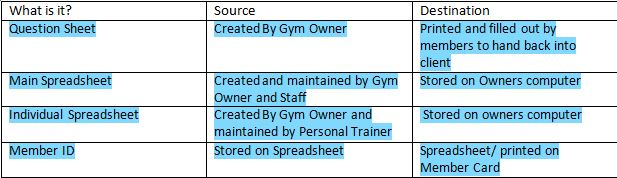
\includegraphics[width=\textwidth]{InvestigationTable1.jpg}
    \caption{Data Sources and Destinations for the current system} \label{fig:Current Destinations}
\end{figure}

\subsubsection{Algorithms}

Hierarchy Charts

Gym Sign Up Process
\begin{python}
1. Information is attained from the client
	1.1 My client gives a form to their client to be promptly filled out
	1.2 The client then hands the sheet back into reception 
	1.3 The information provided on this sheets then enter manually into an excel spreadsheet
	1.4 Do they have an exercise plan? Then the plan is created based on an interview with the client
2.Create Membership Card
	2.1 Make sure all necessary details are correct
	2.2 print Membership card 
\end{python}

Payment Process
\begin{python}
1. Client enters
2. Are they paying upfront?
2.1. Process their payment
2.2. Enter the appropriate information into the correct spreadsheet
2.3 Allow them into the facility
3. Have they payed by direct debit?
3.1. Check to see if the payment went through
3.2. If it did allow them into the facility
3.3 If the payment didnt go through then ask them to pay upfront and return to section 2
3.4 If they refuse to pay ask them to leave
\end{python}

Pseudocode

\begin{python}
Gym Sign Up Process

START

Function GetInfo:
	Client fills out form
	Hands form into gym owner
	Owner enters the information into an excel spreadsheet
	IF they have an exercise plan:
		Owner creates a plan based on an interview with client and enters this into it’s
own spreadsheet
	Owner creates Membership Card
	Owner checks to make sure all the info is correct
	Owner prints membership card and gives it to the new member

GetInfo

END


Payment Process

Start

Function ClientPayment:
	Client enters
	IF paying upfront:
		PayingUpFront
	IF paying by direct debit:
		PayingDirectDebit
	IF they refuse to pay:
		AskThemToLeave

Function PayingUpFront:
	Owner processes payment
	Process their payment
	Enter payment information into the appropriate spreadsheet
	Allow them into the facility

Function PayingDirectDebit:
	Check to see if the payment went through
	IF payment didn’t go through:
		IF they want to pay up front:
			PayingUpFront
		ELSE IF they refuse to pay:
			AskThemToLeave
	ELSE IF the payment did go through:
		Allow them into the facility

Function AskThemToLeave:
	Ask them to leave

ClientPayment 

END
\end{python}

Flow Charts

\begin{figure}[H]
    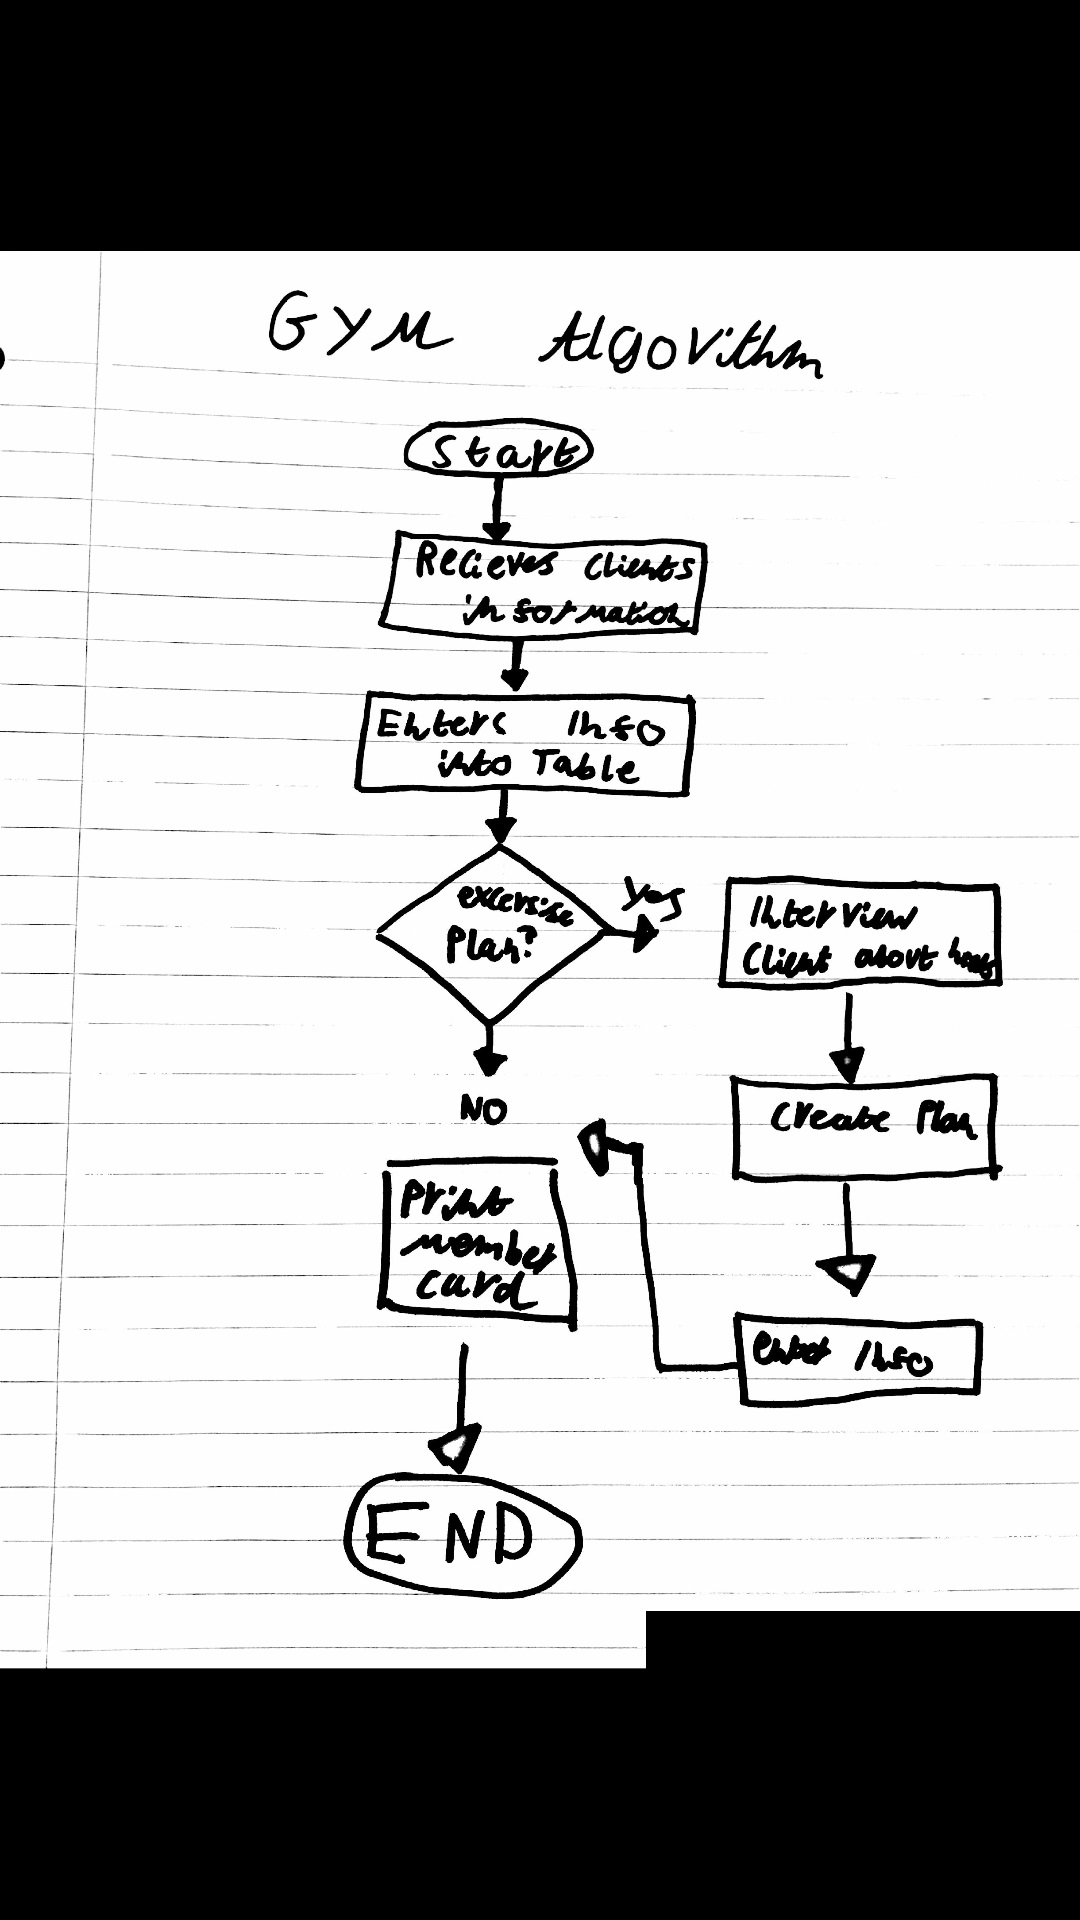
\includegraphics[width=\textwidth]{GymAlgorithm.jpg}
    \caption{Algorithm for the gym sign up process} \label{fig:Algorithm for the gym sign up process}
\end{figure}

\begin{figure}[H]
    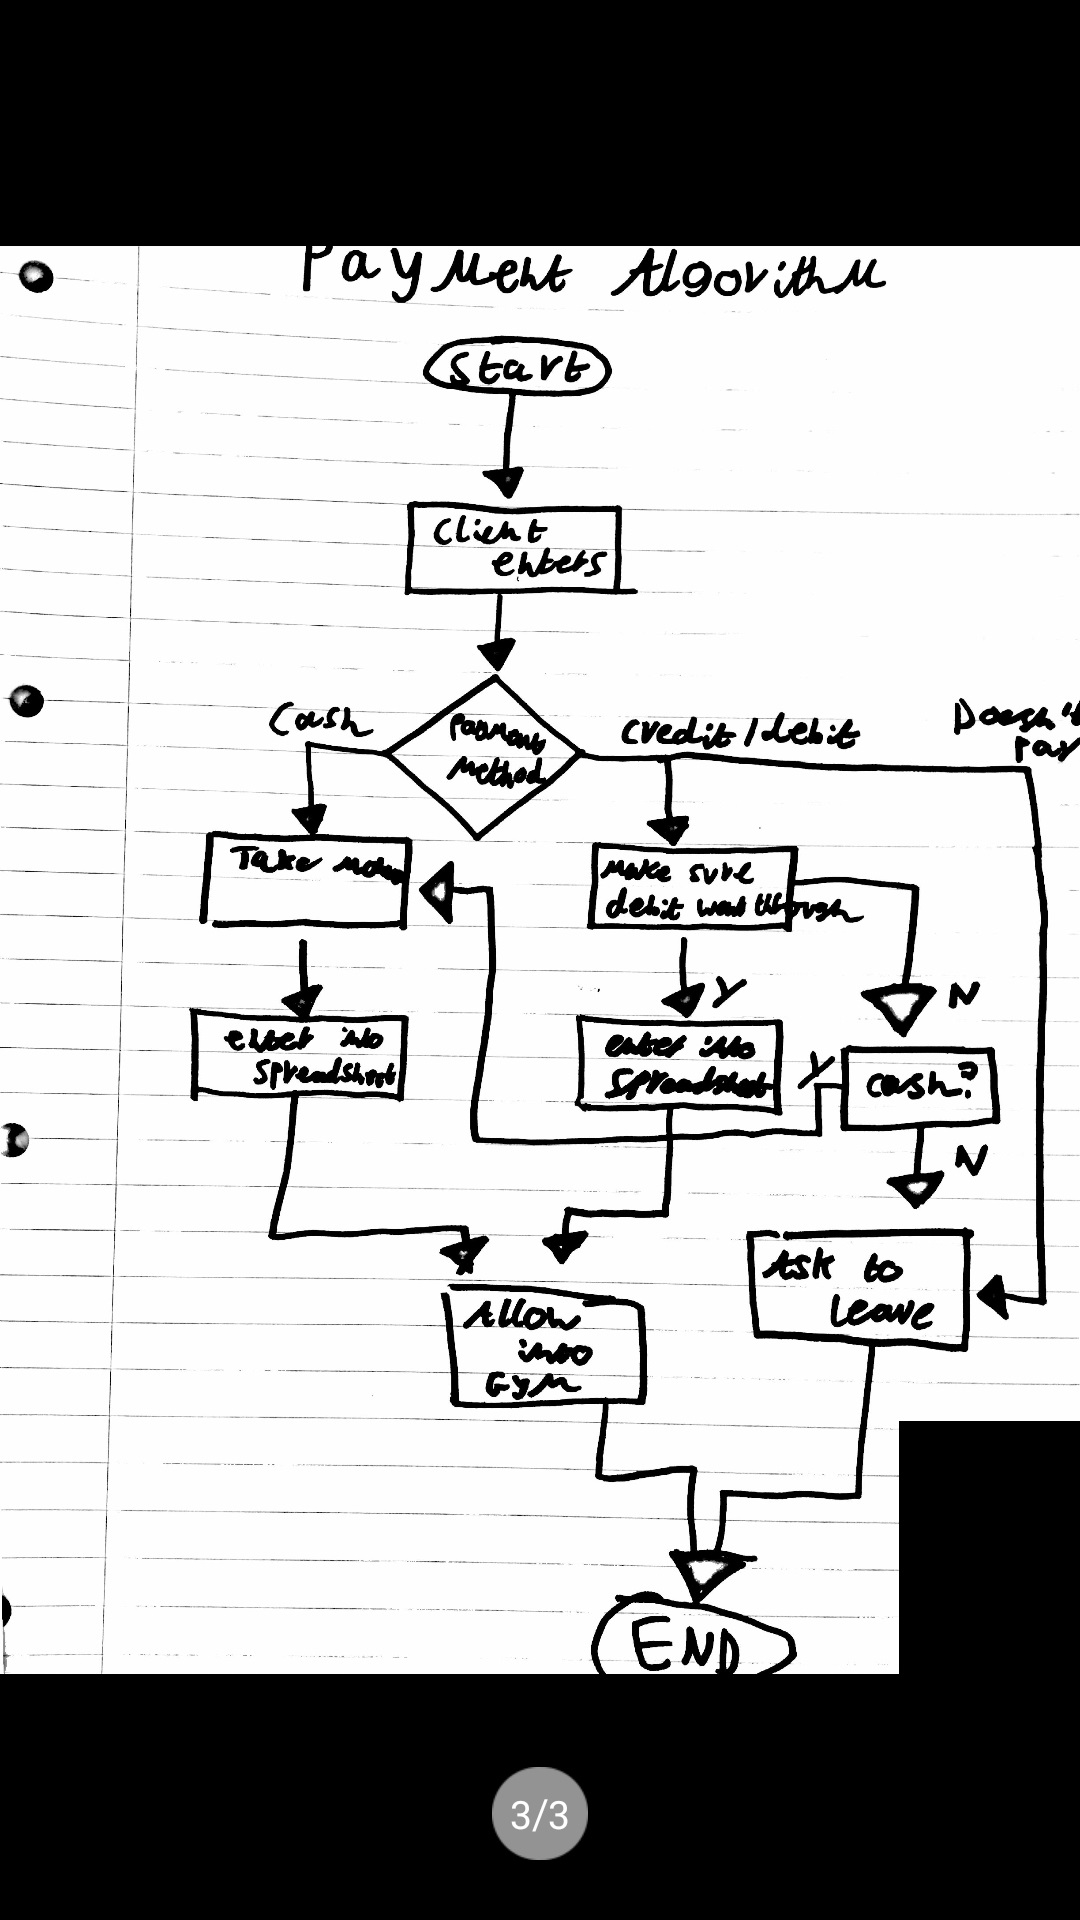
\includegraphics[width=\textwidth]{PaymentAlgorithm.jpg}
    \caption{Algorithm for the payment process} \label{fig:Algorithm for the payment process}
\end{figure}

\subsubsection{Data flow diagram}

\begin{figure}[H]
    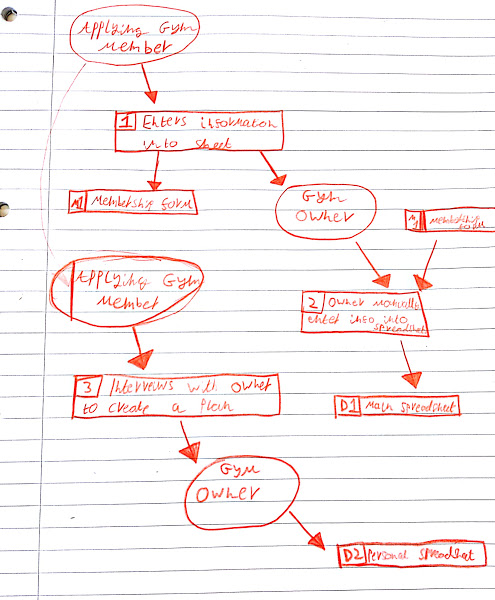
\includegraphics[width=\textwidth]{ProposedDFD.jpg}
    \caption{Data Flow Diagram For The Proposed System} \label{fig:Data Flow Diagram For The Proposed System}
\end{figure}


\subsubsection{Input Forms, Output Forms, Report Formats}

\begin{figure}[H]
    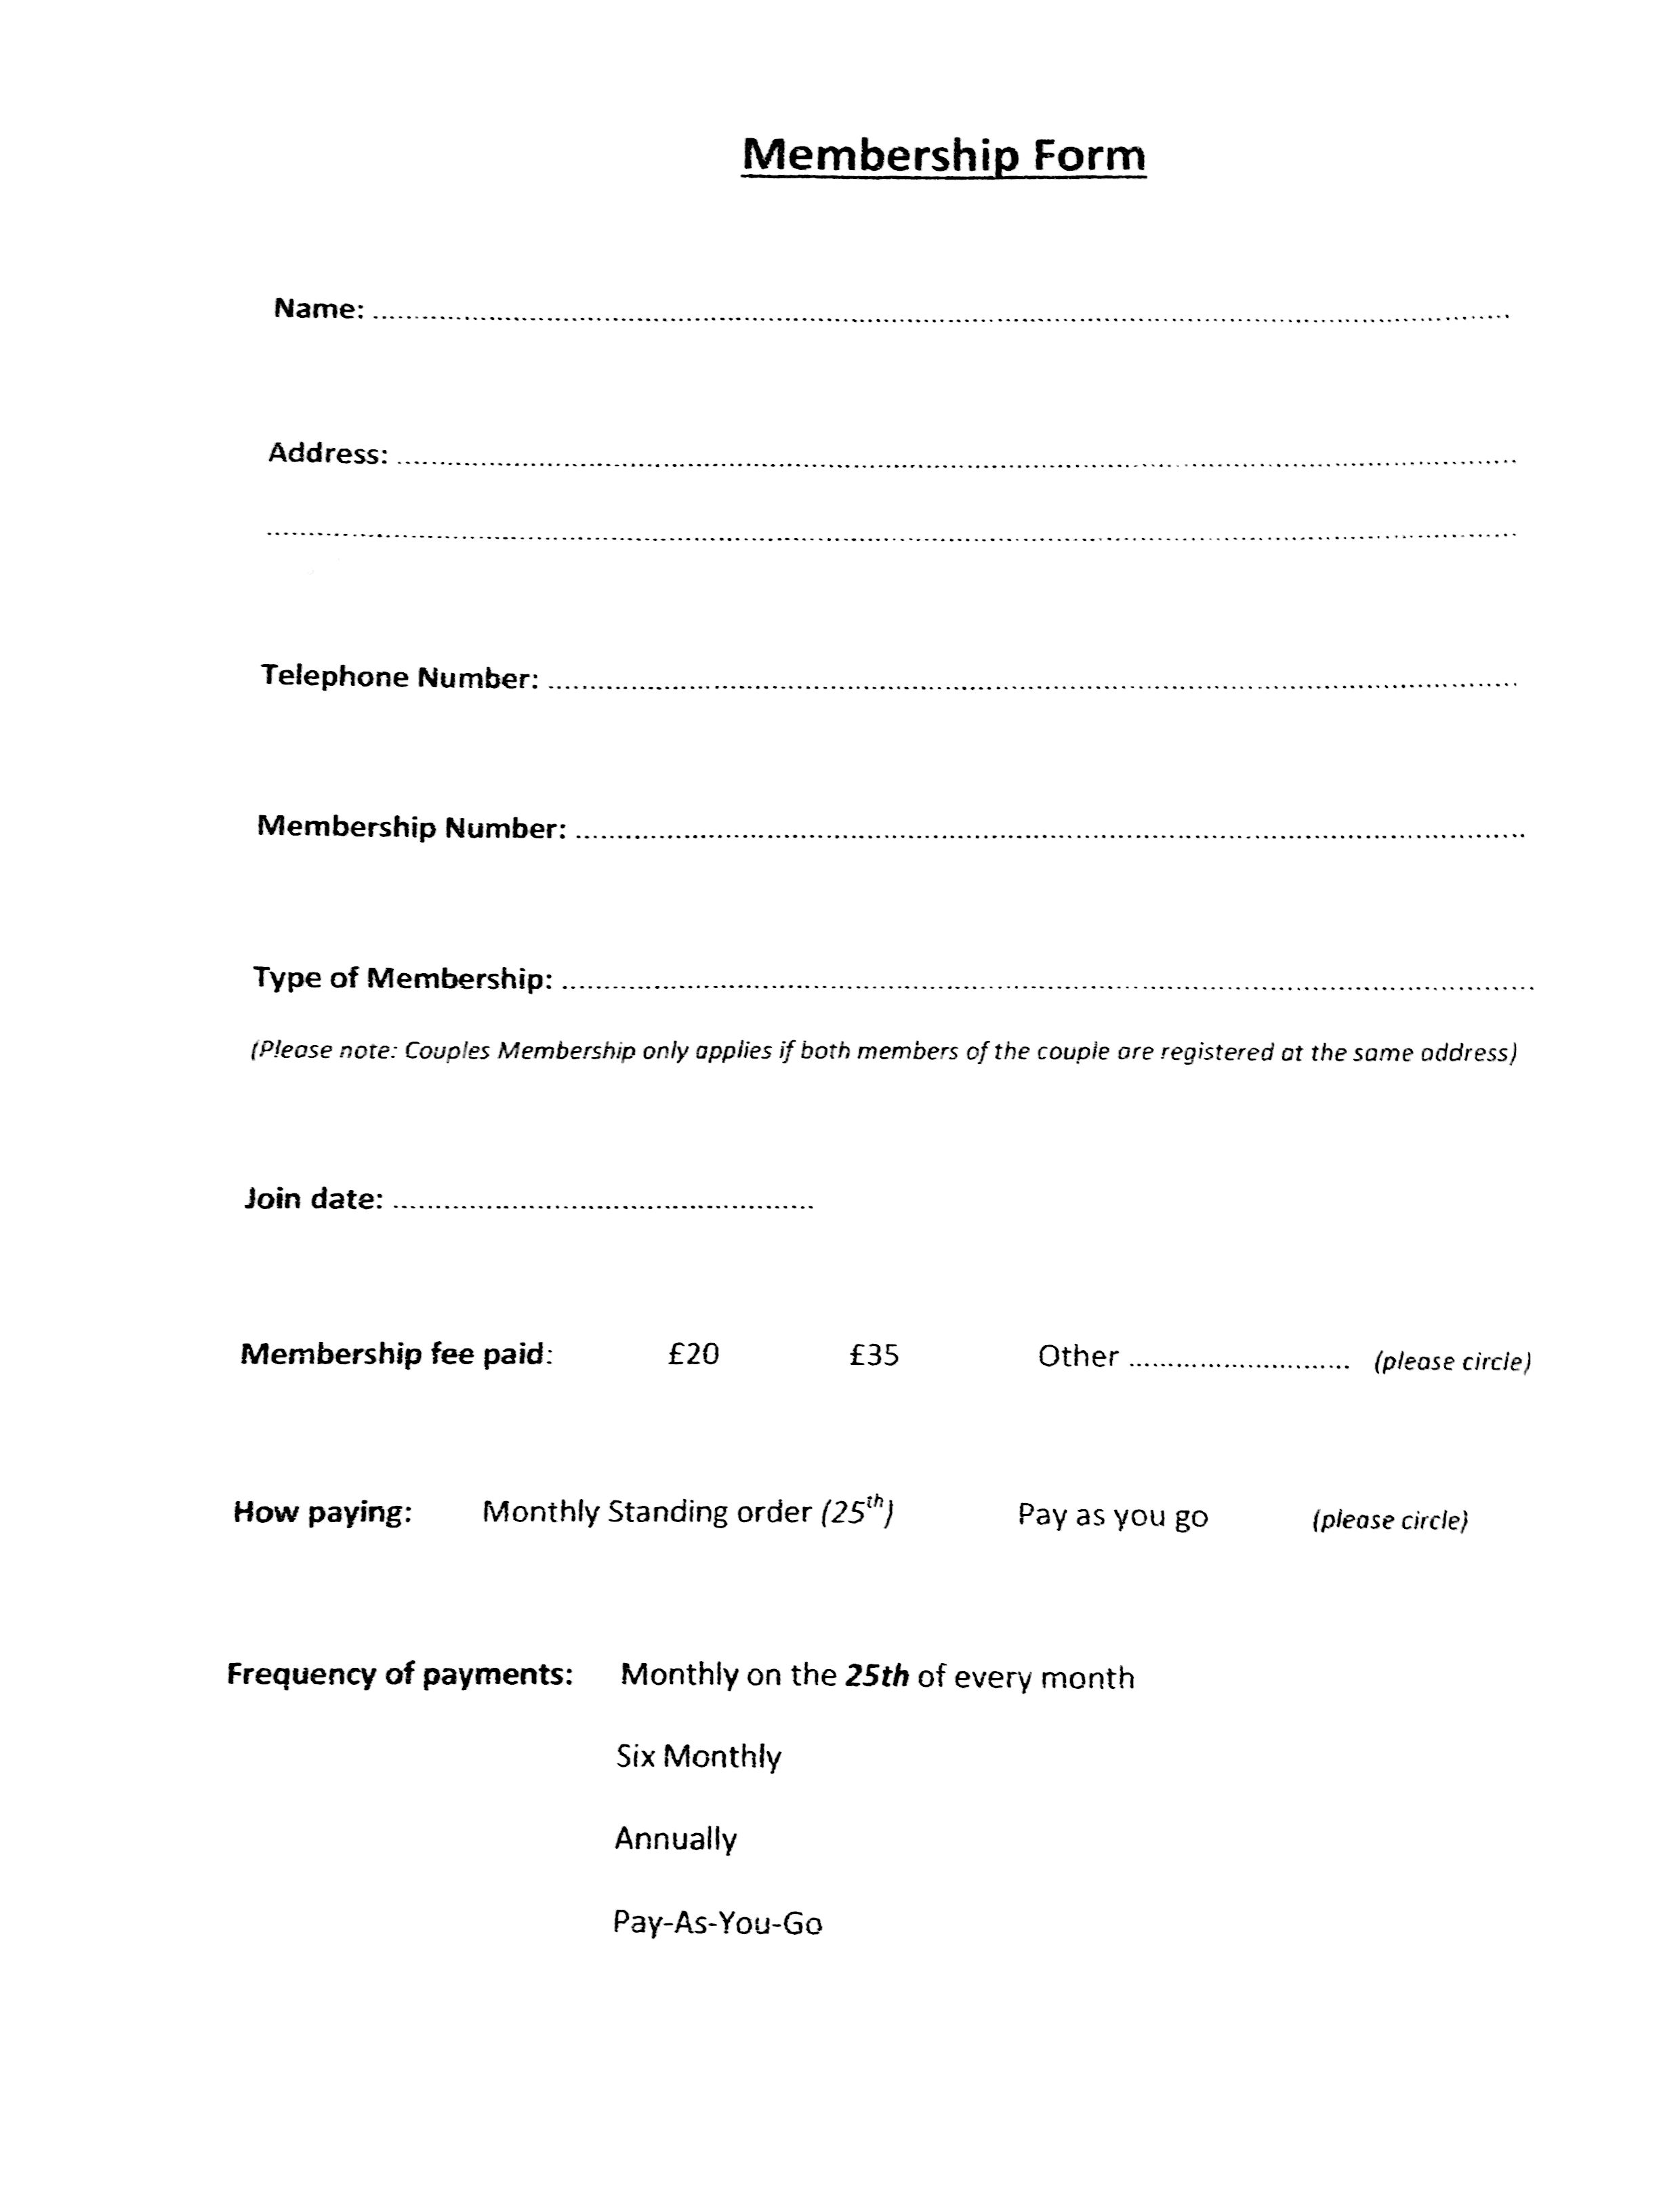
\includegraphics[width=\textwidth]{MembershipForm.jpg}
    \caption{Membership Sign up form} \label{fig:Membership Sign up Form}
\end{figure}

\begin{figure}[H]
    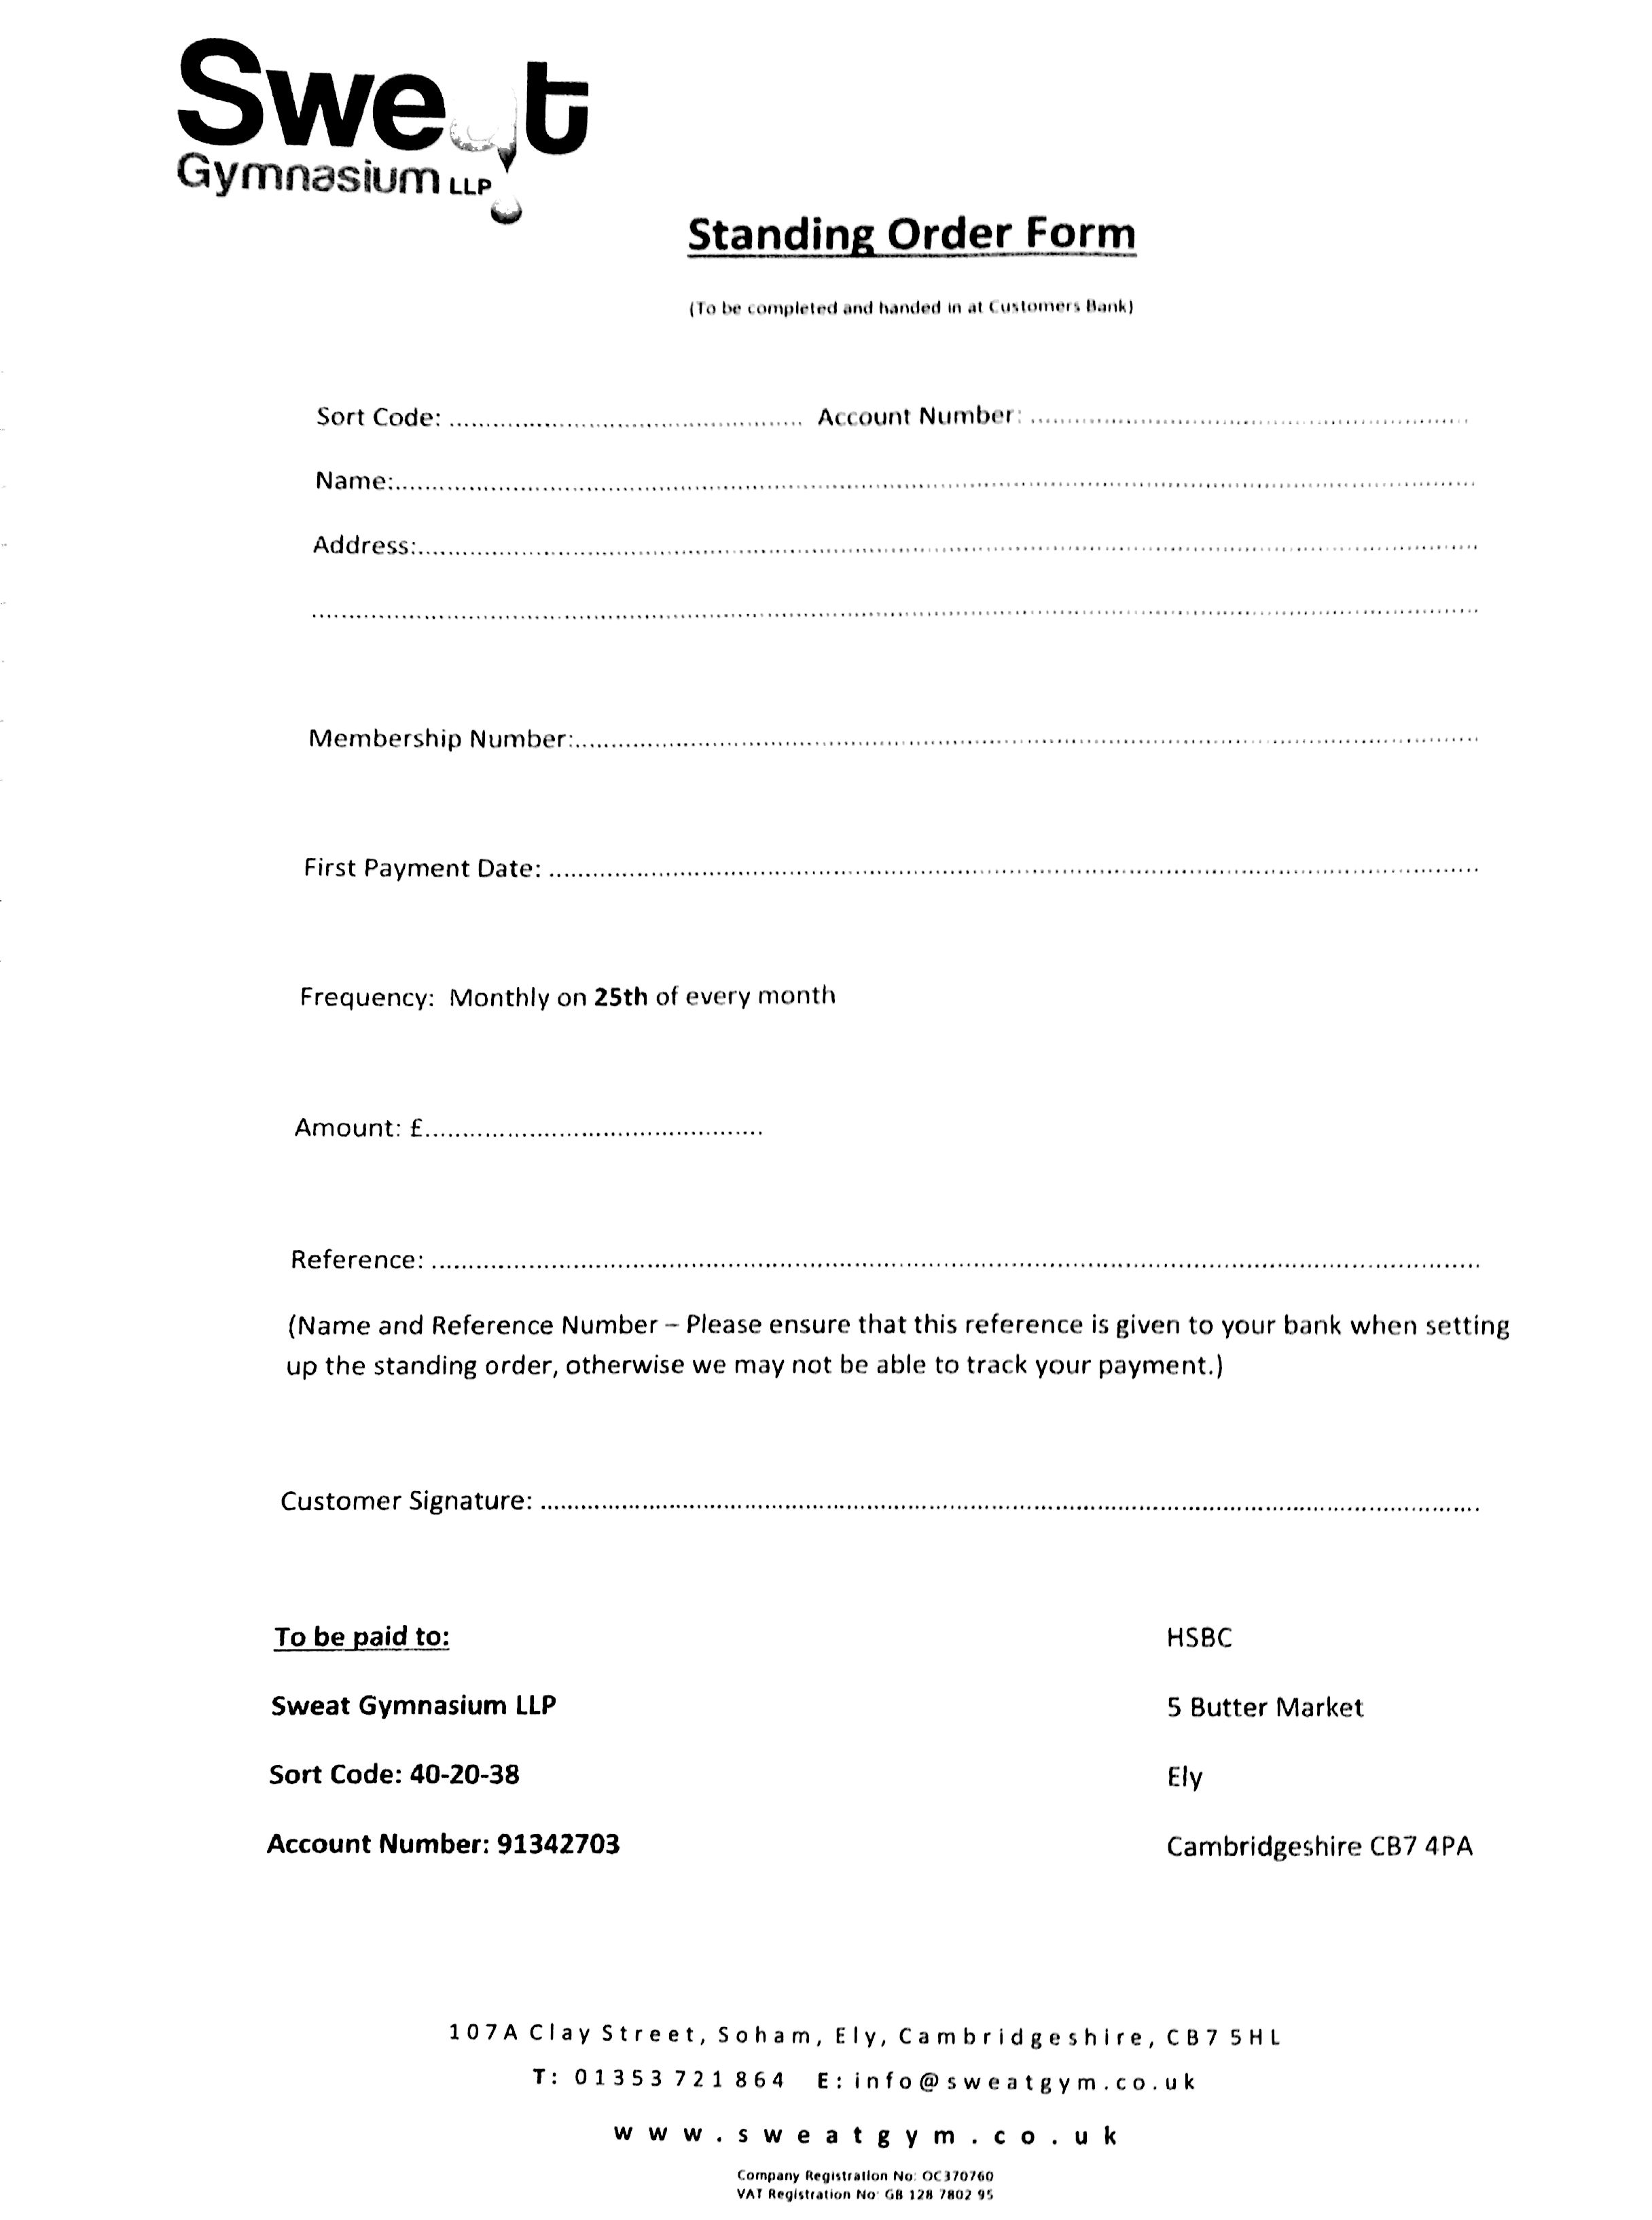
\includegraphics[width=\textwidth]{StandingOrderForm,jpeg.jpg}
    \caption{Standing Order Form} \label{fig:Standing Order Form }
\end{figure}

\subsection{The proposed system}

My proposed system uses a database to keep track of all the data that my client previously kept in an excel spreadsheet using a program created in the python programming language using the PyQt 4 library. This is because its the language I'm most comfortable with and allows for the creation of intuitive UI and the creation of an executable program using the software cx freeze ensuring that the system will be easily usable by my client.

\subsubsection{Data sources and destinations}

\begin{figure}[H]
    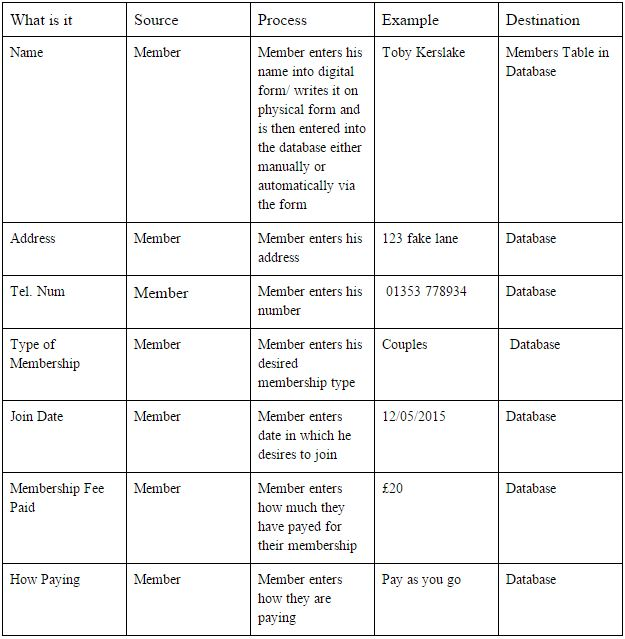
\includegraphics[width=\textwidth]{ProposedSources.jpg}
    \caption{Data Sources and Destinations} \label{fig: Data Sources and Destinations }
\end{figure}

\begin{figure}[H]
    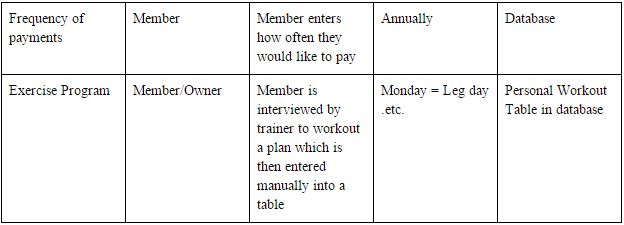
\includegraphics[width=\textwidth]{ProposedSources2.jpg}
    \caption{Data Sources and Destinations 2} \label{fig: Data Sources and Destinations 2 }
\end{figure}

\subsubsection{Data flow diagram}

\begin{figure}[H]
    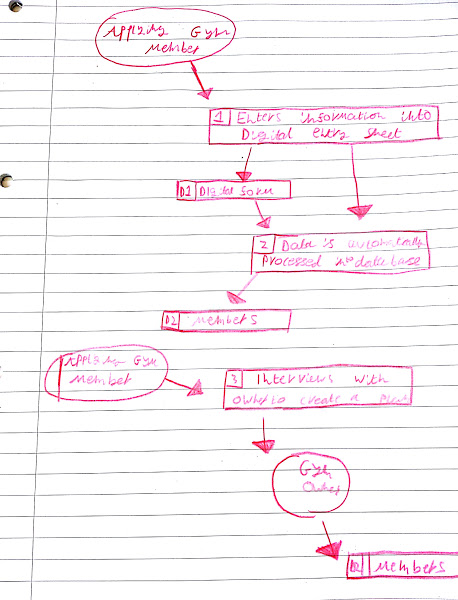
\includegraphics[width=\textwidth]{ProposedDFD2.jpg}
    \caption{Data Flow Diagram} \label{fig: Data Flow Diagram }
\end{figure}

\subsubsection{Data dictionary}

\begin{figure}[H]
    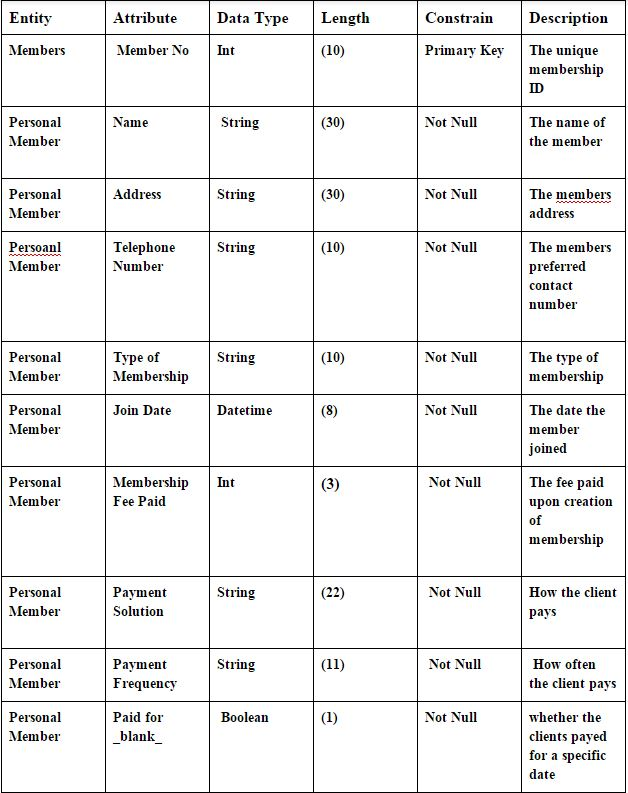
\includegraphics[width=\textwidth]{Sources.jpg}
    \caption{Data Destinations and Sources} \label{fig: Data Destinations and Sources }
\end{figure}

\begin{figure}[H]
    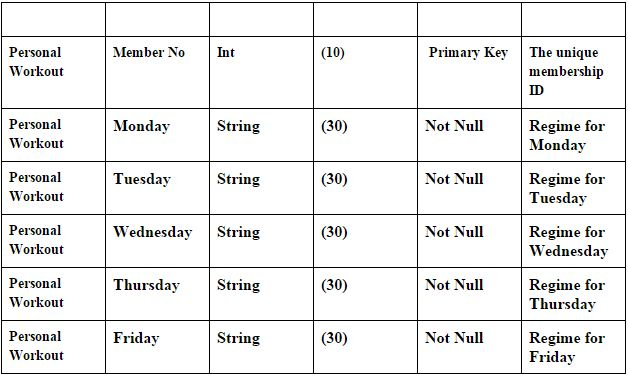
\includegraphics[width=\textwidth]{Sources2.jpg}
    \caption{Data Destinations and Sources 2} \label{fig: Data Destinations and Sources 2 }
\end{figure}

\subsubsection{Volumetrics}

I have decided on an initial size of 2000 members since the gym is nearing that number of members and will inevitably achieve this amount of clients.  My client has said the amount of clients he gains isn't consistent as people often register in different sized groups. The size of the database can be increased at a later date when needed.  

Each member has 11 - 16 fields of data in total, with each data field taking up 1 KB of data.

16 * 1KB * 2000 = 32000 KB
32000 / 1024 = 31.25 MB

The rest of the system should take up a small amount of space that will probably take up about 3MB.

31.25 MB + 3MB = 34.25 MB

\section{Objectives}



\subsection{General Objectives}

\subsection{Specific Objectives}

\subsection{Core Objectives}

\subsection{Other Objectives}

\section{ER Diagrams and Descriptions}

\subsection{ER Diagram}

\subsection{Entity Descriptions}

\section{Object Analysis}

\subsection{Object Listing}

\subsection{Relationship diagrams}

\subsection{Class definitions}

\section{Other Abstractions and Graphs}

\section{Constraints}

\subsection{Hardware}

\subsection{Software}

\subsection{Time}

\subsection{User Knowledge}

\subsection{Access restrictions}

\section{Limitations}

\subsection{Areas which will not be included in computerisation}

\subsection{Areas considered for future computerisation}

\section{Solutions}

\subsection{Alternative solutions}

\subsection{Justification of chosen solution}